\documentclass[12pt]{article}

\usepackage{graphicx}
\usepackage{cmsrb}
\usepackage[OT2,T1]{fontenc} %better to use T1, but OT1 will also work
\usepackage[serbian]{babel}
\usepackage[utf8]{inputenc}
\usepackage[a4paper,top=2cm,bottom=2cm,left=3cm,right=3cm,marginparwidth=1.75cm]{geometry}
\usepackage{times}

	

\usepackage[colorlinks=true, allcolors=blue]{hyperref}

\begin{document}
\title{ИТ конференције у Србији 2022. године\\ \small{Seminarski rad u okviru kursa\\Tehničko i naučno pisanje\\ Matematički fakultet}}
\author{Невена Јокић\\ nevenajokic2003@gmail.com \and Андреј Михајлов\\ andrejm17@gmail.com \and Душан Лукић\\ mejl \and Јован Гагић\\ jovangagiccofi@gmail.com}
\date{23.~avgust 2023.}
\maketitle
\abstract{Овај рад анализира улогу и допринос конференција, посебно ИТ конференција, у данашњем друштву у Србији и у свету.}

\newpage

\tableofcontents
\newpage

\section{Увод}

Конференције су планирани догађаји на којима се професионалци или стручњаци окупљају како би поделили знање, разменили идеје и повезали се са другима у истој области. Ове прилике се често дешавају у различитим областима и секторима, као што су технологија, наука, медицина, бизнис, образовање, уметност и другe. Појам конферфенција оригинално потиче из латинског језика од речи \textit{conferentia} што значи састанак или окупљање. За сазивање конференције није потребна никаква традиција, континуитет или периодичност конференције. Иако углавном нису временски ограничене, конференције су обично кратког трајања
са специфичним циљевима. Због сличности у именима долази до мешања са конвенцијама, али конвенције су у већини случајева доста већи догађаји који се састоје од делегација које представљају различите групе.
Скупови, састанци и догађаји били су део живота људи од најраније забележене историје. Археолози су пронашли примитивне рушевине од давнина културе које су се користиле као простори за састанке где би се грађани окупљали да разговарају о заједничким интересима, као што су влада, рат, лов или племенске прославе. Једном када људи развију отворена стална насеља, сваки град или село је имао јавни простор за састанке, који се често звао градски трг, где су се становници могли састати, разговарати и прославити. Прва позната употеба речи конфереција се појављује у 16. веку, међутим идеја о конференцији се појавила далеко пре употребе. 
Конференције могу имати различите формате, теме и намере. Што се тиче формата конференције разликујемо следеће:
\begin{enumerate}
    \item Конференцијски позив – у телекомуникацијама, представља позив од два или више учесника у исто време. Први забележен конференцијски позив oбавио је 1915. године Александар Бел, први власник патента за телефон у Сједињеним Америчким Државама. Његов помоћник Вотсон, као и градоначелници Њујорка и Сан Франциска, придружили су се Белу на првом конференцијском позиву 1915.
    \item Конференцијске сале – сале и просторије у којима се одржавају конференције.
    \item Видео конференције – конференције које се одвијају преко аудио-видео позива са учесницима на различитим локацијама. Током пандемије вируса ковид-19, видео конференције су постале веома популарне и неопходне да би нека конференција могла да се одржи. Међутим, њихова популарност се одржала и наставила да расте чак и након проглашења завршетка пандемије.
\end{enumerate}
На конференцијама се расправља о иновативним идејама и размењују се нове информације међу стручњацима. По намери конференција разликујемо следеће:
\begin{enumerate}
    \item Пословне конференције – конференције које се одржавају за исту компанију или индустрију. Стручњаци се окупљају да би дискутовали о новим приликама које се тичу њиховог посла.
    \item Академске конференције – конференције на којима се окупљају научници или академици који презентују своја истраживања о којима се затим дискутује.
    \item Трговинска конференција – конференције већег обима на којима се поред бизнисмена и привредника скупљају и грађани који долазе да се повежу са продавцима и остваре нове везе.
    \item Некоференција – конференција која избегава велике трошкове и спонзорисане презентације. Сви учесници су једнако упућени у тему конференције и дискусија је отвореног типа тојест некоференције углавном немају једног главног говорника који се обраћа скупу.
\end{enumerate}

\pagebreak

\section{ИТ конференције}
Информационе технологије или скраћено ИТ представљају дисциплину која подразумева коришћење рачунара за складишћење, анализу, преузимање, пренос и манипулацију података или информација. Термин информационе технологије се користи у много ширем смислу који подразумева све активности којима се ИТ стручњаци баве, од инсталација апликативних програма до пројектовања сложених рачунарских мрежа.
ИТ конференције су конференције које за циљ имају да окупе стручњаке и истраживаче из поља информационих технологија као и људе који желе да науче више о њима. Учесници се окупљају да дискусују о новим идејама, трендовима и развоју ИТ сектора. Постоје стотине релевантних подтема у овој области као што су сајбер безбедност, виртуелна реалност, вештачка интелигенција и машинско учење, технолошко планирање за унапређење образовања, дигиталне технологије и још много тога. Величина и фокус конференција о информационим технологијама могу варирати. Неке се дешавају лично, док су неке виртуелне. ИТ конференције учесницима дају могућност умрежавања са другим професионалцима како би унапредили своју каријеру и пословање као и искуство из прве руке са најновијим алатима и технологијама у овој области.
\subsection{ИТ конференције у Србији}
Србија, као земља која све више препознаје потенцијал информационих технологија, постала је и 2022. године домаћин разноврсним и великим ИТ конференцијама које су окупиле стручњаке и знатижељне из целог света. Међу огромним бројем конференција које су се одржале те године највише су се истакле: Синергија, “COMING IT” конференција, TMRW Belgrade конференција, OpenIt, Telfor konferencija, Data Science konferencija.

\subsection{TELFOR 2022}
ТЕЛФОР, односно телекомуникациони форум, је годишњи интернационални скуп стручњака из области информационих технологија и телекомуникација. Учесници су најчешће телекомуникациони инжењери, али такође и правници, менаџери, економисти, оператори и други. На ТЕЛФОР-у се разматрају сва релевантна питања телекомуникација: техничка, регулаторна, економска и развојна, питања производње опреме, услуга, сервиса и функционисања система.
У току ТЕЛФОР-а организују се:
\begin{itemize}
	\item стручне и комерцијалне презентације компанија,
	\item сесије са радовима студената редовних и мастер студија,
	\item изложба телекомуникационог хардвера, софтвера, система, пратеће опреме и услуга, 
	\item презентације нових стручних књига,
	\item образовни семинари за младе стручњаке и студенте редовних и мастер студија,
	\item презентације и скупови професионалних удружења, конференције за штампу, пријеми, итд. 
	\item стручни семинари за афирмисане стручњаке, 
	\item више десетина ауторских сесија са ауторским радовима из различитих области телекомуникација, 
	\item специјалне презентације водећих интернационалних и домаћих телекомуникационих компанија,
	\item пленарне седнице са предавањима по позиву,
	\item тематске расправе, панел дискусије и округли столови у вези са актуелним темама,
\end{itemize}

Значај ТЕЛФОР-а за телекомуникацију расте сваке године. ТЕЛФОР већ годинама има велик број учесника и посетилаца из свих телекомуникационих сегмената. Око 2000 посетилаца долази на ТЕЛФОР и прихвата се од 300-500 детаљно рецензираних радова са укупно 700-900 аутора/коаутора. Мноштво телекомуникационих компанија сваке године сарађују са ТЕЛФОР-ом, међу којим су Agilent, Alcatel, Cisco, Ericsson, HP, Huawey, IBM, Intracom, Juniper, Microsoft, Motorola, Rohde And Schwarz, Siemens и друге, по правилу заједно са својим локалним партнерима, као и око 50 домаћих и међународних организација донатора и учесника.\cite{telfor}

\subsection{Синергија 2022}
Синергија је једна од највећих и најутицајнијих конференција у Југоисточној Европи посвећена дигиталној трансформацији. Организује је Microsoft Србија и одржава се већ 22 године. 2022. године слоган је био “Speed it up”. Трајала је три дана oд 6. до 8. децембра 2022. године и била је подељена по следећим сегментима: технички дан, бизнис дан, ЕДУ синергија, Women know it и синергија журка.

\begin{figure}[h!]
        \centering
\includegraphics[height=2.5cm]{slike/sinergija.jpg} 
        \caption{Promo slika za Sinergiju 22}
        \label{fig:sinergija22}
\end{figure}

Синергија обухвата широк спектар тема, међутим 2022. главне теме су биле како технологија данас покреће светску економију, технолошка трансформација образовања, континуална дигитализација, енергетска ефикасност и модерно пословање. Као и прошлих година, и ове године синергија је окупила стручњаке и саговорнике из државних институција и најуспешнијих компанија у Србији и Југоисточној Европи. У табели \ref{tab:tabela1} су приказане статистике за синергију 22, односно колико је било излагача, постеилаца и величина изложбеног простора.\cite{sinergija}

\begin{table}[h!]
\begin{center}
\begin{tabular}{|ccc|} \hline
\multicolumn{3}{|c|}{Статистике за синергију 22}                                                                  \\ \hline
\multicolumn{1}{|c|}{Број излагача} & \multicolumn{1}{c|}{Број посетилаца}          & Изложбени простор           \\ \hline
\multicolumn{1}{|c|}{Преко 90}      & \multicolumn{1}{c|}{Преко 2000 рекордни број} & 1500м2 Crowne plaza Beograd \\ \hline
\end{tabular}
\caption{Statistika za Sinergiju 22}
\label{tab:tabela1}
\end{center}
\end{table}

\subsection{TMRW Belgrade конференција}

TMRW конференција је једна од највећих технолошких догађаја у успону у Европи која окупља преко 40000 учесника, како уживо тако и онлине, као и преко 100 говорника и презентатора. Главна тема ове конференције је истраживање најновијих трендова у областима вештачке интелигенције, блокчејна, криптовалута, НФТ -ја, метаверс-а и гејминга као и упознавање учесника са истим.  

Београд је од 13. до 15. маја 2022. године био домаћин овог огромног догађаја. Церемонија отварања била је представљена као футуристички спетакл, уз специјалне ефекте, ласере и пиротехнику. Поред учења о развоју и “рударењу” криптовалута, постеиоци су имали прилику и да упознају људе који су креирали неке од најистакнутијих НФТ пројеката. TMRW 2022 конференција је окупила водеће светске блокчејн компаније и утицајне стручњаке. Присутни су такође имали шансу да упознају пионире Метаверс-а који су их едуковали о потенцијалу и утицају ове технологије на наше животе и свет какав познајемо. На конференцији је било више од 50 говорника и уводних излагања са бројним интерактивним дисусијама и радионицама. У табели \ref{tab:tabela2} су приказане статистике за TMRW Belgrade 2022, односно колико је било излагача, постеилаца и величина изложбеног простора.\cite{tmrw}

\begin{table}[h!]
\begin{center}
\begin{tabular}{|ccc|}
\hline
\multicolumn{3}{|c|}{Статистике за TMRW конференцију}                                                                  \\ \hline
\multicolumn{1}{|c|}{Број излагача} & \multicolumn{1}{c|}{Број посетилаца}          & Изложбени простор           \\ \hline
\multicolumn{1}{|c|}{Преко 50}      & \multicolumn{1}{c|}{Преко 21000 уживо и онлине} & 2500м2 Belexpo centar \\ \hline
\end{tabular}
\caption{Statistika za TMRW Belgrade 2022}
\label{tab:tabela2}
\end{center}
\end{table}
 
\subsection{19. COMING IT конференција}
Компанија COMING (Computer Engineering d.o.o.), један од лидера у ICT (Information and Communications) области у Србији и региону, је компанија која поставља за циљ креирање, развијање и пружање ИТ система и услуга. 25. октобра 2022. године организовали су своју 19. ИТ конференцију. Главна тема ове конференције је била усмерена ка размишљању на питање како ИТ функција може бити организована, а да се обезбеди фокус на главни бизнис и потребну агилност у пословању.\cite{comingit}

\subsection{Data Science Conference 2022}
DataScienceConference је интернационална AI и Data конференција у Београду која пружа најсавременије увиде у AI и Data Science. 2022. године је било преко 200 говора и 50 tech туторијала. 

\begin{figure}[h!]
        \centering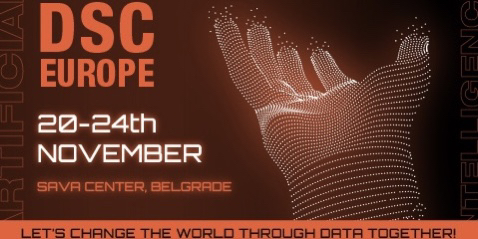
\includegraphics[height=2.5cm]{slike/dsc.jpg} 
        \caption{Promo slika za Data Science Conference 2022}
        \label{fig:dsc22}
\end{figure}

DSC окупља више од 3000 најутицајнијих и најобразованијих стручњака у индустрији на тродневни догађај пун дискусија, панела, пословних прилика и доживотног знања. Говорници на овој конференцији долазе из неких од најутицајнијих ИТ компанија на свету попут Google, IBM, VMWare i EyeSee.\cite{dsc}

\subsection{Open IT}
Open IT је највећа ИТ конференција за младе. Преко 17 година помажу студентима да развију своје каријере, тако што им дају прилику да развију своја интересовања у различитм сферама ИТ-а, упознају се са понудом пракси/послова и чују приче најуспешнијих личности и компанија.

У два дана конференције на једном месту окупљају 350+ младих, 10+ говорника и 40+ предавача из 20+ компанија.\cite{openit}

\section{Закључак}
Конференције су постале важан део друштва и професионалног развоја компанија, посла и људи. Омогућавају учесницима да се повежу са стручњацима и колегама из целог света. Размењују се мишљења, идеје, искуства, научни радови и још много других ствари које помажу појединцима у изградњи односа и нових технологија.Србија, иако не спада међу велике државе, је свеједно често домаћин великим ИТ дешавањима и конференцијама. Стотине људи, а поготово млади, из региона и света долазе у Београд да учествују у разним ИТ радионицама које ове конференције организују.

\pagebreak

\addcontentsline{toc}{section}{Literatura}
\appendix

\iffalse
\bibliography{seminarski}
\bibliographystyle{plain}
\fi

\begin{thebibliography}{9}
\bibitem{telfor} \emph{TELFOR 2022} \url{https://2022.telfor.rs/sr/} 15.11.2022.

\bibitem{sinergija} \emph{Sinergija 2022} \url{https://www.stat.gov.rs/vesti/20221209-najveca-regionalna-it-konferencija-odrzana-u-beogradu-sinergija-2022/} 9.12.2022.

\bibitem{tmrw} \emph{TMRW Belgrade 2022} \url{https://tmrwconf.net/tmrw-conference-2022/} 23.06.2022.

\bibitem{comingit} \emph{COMING IT}.\url{https://konferencija.coming.rs/} 25.10.2022.


\bibitem{dsc} \emph{Data Science Conference 2022} \url{https://datasciconference.com/} 20.11.2022.

\bibitem{openit} \emph{OPEN IT} \url{https://open-it.rs/} 30.11.2022.

\end{thebibliography}

\appendix

\end{document}
